\documentclass[aspectratio=169,11pt]{beamer}

\usetheme{default}
\usecolortheme{default}
\usefonttheme{professionalfonts}
\usepackage[T1]{fontenc}
\usepackage{lmodern}
\usepackage{booktabs}
\usepackage{tikz}
\usetikzlibrary{arrows.meta,positioning}

\definecolor{accent}{HTML}{2A78D6}
\definecolor{ink}{HTML}{0B0B0B}
\definecolor{muted}{HTML}{52514E}
\definecolor{boxblue}{HTML}{E8F1FC}
\setbeamercolor{frametitle}{fg=accent}
\setbeamercolor{title}{fg=accent}
\setbeamercolor{normal text}{fg=ink}
\setbeamercolor{itemize item}{fg=accent}
\setbeamercolor{itemize subitem}{fg=muted}
\setbeamercolor{enumerate item}{fg=accent}
\setbeamertemplate{navigation symbols}{}
\setbeamertemplate{itemize items}[circle]
\setbeamerfont{frametitle}{series=\bfseries,size=\Large}
\setbeamertemplate{footline}{\hfill\textcolor{muted}{\scriptsize Krishna Jhanwar --- PrefEval mid-term \quad \insertframenumber/\inserttotalframenumber}\hspace{0.4cm}\vspace{0.25cm}}

\newcommand{\nQuestions}{64,535}
\newcommand{\nCells}{65}
\newcommand{\nQuestionsRun}{64,478}
\newcommand{\gpuHours}{71}
\newcommand{\nCompared}{29}
\newcommand{\nWithinFive}{12}
\newcommand{\nWithinTen}{20}
\newcommand{\medianAbsDelta}{6.0}
\newcommand{\llamaSCemptyOneK}{25.2}
\newcommand{\llamaSCrtwZero}{205}
\newcommand{\llamaSCwtrZero}{51}
\newcommand{\llamaSCfirstZero}{94.4}
\newcommand{\mistralSCrtwZero}{188}
\newcommand{\mistralSCwtrZero}{29}
\newcommand{\mistralSCfirstZero}{95.6}
\newcommand{\posAccAthree}{60}
\newcommand{\posAccDthree}{43}
\newcommand{\posAccAlong}{42}
\newcommand{\posAccDlong}{23}
\newcommand{\posPickDthree}{14}
\newcommand{\posPickDlong}{8}
\newcommand{\llamaRagRefusalAll}{19.1}

\graphicspath{{figures/}}

\newcommand{\takeaway}[1]{\vspace{4pt}\begin{beamercolorbox}[sep=6pt,rounded=true]{normal text}\colorbox{boxblue}{\parbox{0.93\linewidth}{\small #1}}\end{beamercolorbox}}

\title{Improving Long-Context Preference Following in LLMs}
\subtitle{Mid-term: Phase 1, reproducing PrefEval baselines on local models}
\author{Krishna Jhanwar (12341250)}
\date{October 2026}

\begin{document}

\begin{frame}[plain]
\titlepage
\end{frame}

%-------------------------------------------------------------------------------
\begin{frame}{The problem and the plan}
\begin{columns}[T]
\begin{column}{0.5\textwidth}
\textbf{Problem} (PrefEval, ICLR 2025)
\begin{itemize}
  \item A user states a preference early (\emph{``I avoid gluten''})
  \item Unrelated conversation follows
  \item Later query: \emph{``Restaurants in Rome?''}
  \item LLMs often forget the preference as context grows
\end{itemize}
\end{column}
\begin{column}{0.5\textwidth}
\textbf{Three phases}
\begin{enumerate}
  \item \textbf{Reproduce baselines} \hfill \textcolor{accent}{\textbf{done}}
  \item Train a preference-detection classifier
  \item Classifier $\rightarrow$ preference memory + modern retriever, compared against the Phase~1 baselines
\end{enumerate}
\end{column}
\end{columns}
\takeaway{This talk covers Phase 1: \nQuestions{} questions, 2 models, 5 methods, 2 preference forms, 0.2k--23k tokens, about \gpuHours{} GPU-hours on one RTX 3060.}
\end{frame}

%-------------------------------------------------------------------------------
\begin{frame}{The benchmark task (classification)}
\begin{itemize}
  \item 1{,}000 preference--query pairs, 20 topics, explicit and implicit preference forms
  \item Preference at the start $\rightarrow$ \texttt{inter\_turns} unrelated LMSYS turns $\rightarrow$ query with 4 options
  \item Exactly one option respects the preference; metric = accuracy averaged over 20 topics
\end{itemize}
\vspace{4pt}
\textbf{Five baselines}
\begin{itemize}
  \item \textbf{Zero-shot}: answer directly
  \item \textbf{Reminder}: one sentence asking the model to consider earlier preferences
  \item \textbf{CoT}: five worked examples of preference-aware answers
  \item \textbf{Self-Critic}: answer $\rightarrow$ critique $\rightarrow$ revised answer
  \item \textbf{RAG}: top-5 past exchanges retrieved with SimCSE and quoted before the question
\end{itemize}
\end{frame}

%-------------------------------------------------------------------------------
\begin{frame}{Constraint: no Bedrock, one 12\,GB GPU}
\begin{columns}[T]
\begin{column}{0.55\textwidth}
\textbf{Models from the paper, served locally (Ollama, 8-bit)}
\begin{itemize}
  \item \textbf{Llama-3-8B-Instruct}: 8k context $\rightarrow$ 0.2k--3k rows
  \item \textbf{Mistral-7B-Instruct-v0.2}: 32k context $\rightarrow$ up to 23k tokens (the proposal's long regime)
  \item Greedy decoding (temperature 0, seed 41)
\end{itemize}
\textbf{Ruled out}
\begin{itemize}
  \item Mixtral-8x7B / 70B models: 28+\,GB, exceeds GPU + RAM
\end{itemize}
\end{column}
\begin{column}{0.45\textwidth}
\centering\scriptsize
\resizebox{\linewidth}{!}{\begin{tabular}{rrrrr}
\toprule
Paper row & Paper turns & \texttt{inter\_turns} & Llama-3 tokens & Mistral tokens \\
\midrule
0.2k & 2 & 0 & 275 & 309 \\
1k & 5 & 3 & 1,437 & 1,764 \\
3k & 10 & 8 & 3,282 & 4,023 \\
10k & 30 & 28 & -- (8k limit) & 12,139 \\
16k & 50 & 48 & -- (8k limit) & 19,452 \\
23k & 70 & 68 & -- (8k limit) & 26,878 \\
\bottomrule
\end{tabular}
}\\[4pt]
{\footnotesize Paper rows mapped to \texttt{inter\_turns}, with measured prompt tokens}
\end{column}
\end{columns}
\end{frame}

%-------------------------------------------------------------------------------
\begin{frame}{Pipeline: original prompts, local inference}
\centering
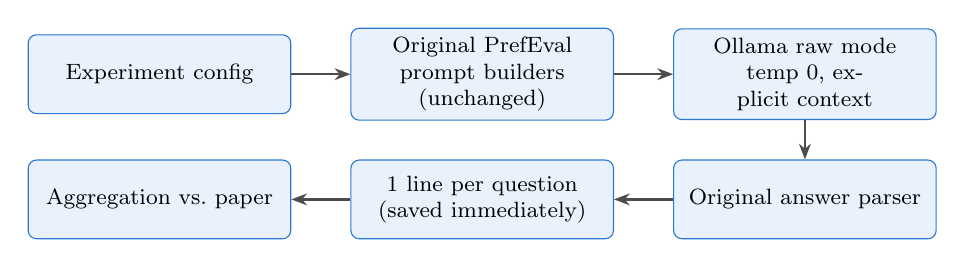
\begin{tikzpicture}[node distance=0.5cm and 0.75cm, font=\footnotesize,
  box/.style={draw=accent, fill=boxblue, rounded corners=3pt, align=center, minimum height=1.0cm, text width=3.1cm},
  arr/.style={-{Stealth[length=2mm]}, thick, color=black!70}]
\node[box] (cfg) {Experiment config};
\node[box, right=of cfg] (up) {Original PrefEval\\prompt builders (unchanged)};
\node[box, right=of up] (oll) {Ollama raw mode\\temp 0, explicit context};
\node[box, below=of oll] (parse) {Original answer parser};
\node[box, left=of parse] (res) {1 line per question\\(saved immediately)};
\node[box, left=of res] (agg) {Aggregation vs.\ paper};
\draw[arr] (cfg)--(up); \draw[arr] (up)--(oll); \draw[arr] (oll)--(parse); \draw[arr] (parse)--(res); \draw[arr] (res)--(agg);
\end{tikzpicture}
\vspace{8pt}
\begin{itemize}
  \item Only the inference call is replaced; prompt text is identical to the authors' code
  \item Resumable after any crash (at most 1 question lost); run manifest with git commit, model digest, settings
  \item A guard refuses runs whose server settings differ from a model's baselines, which keeps Phase~3 comparisons fair
\end{itemize}
\end{frame}

%-------------------------------------------------------------------------------
\begin{frame}{Issues found and fixed (each would have biased the results)}
\small
\begin{enumerate}\setlength{\itemsep}{0pt}
  \item \textbf{First attempt failed}: Gemini import, a missing \texttt{import random}, three copies of \texttt{generate\_message}
  \item \textbf{Double start token}: original prompt + Ollama each add BOS (verified via token counts) $\rightarrow$ stripped
  \item \textbf{Empty self-critiques (Llama)}: indented template ends in whitespace $\rightarrow$ model stops at once $\rightarrow$ trimmed
  \item \textbf{Silent truncation}: Ollama cuts long prompts \emph{from the start}, where the preference is $\rightarrow$ explicit context size and checks
  \item \textbf{Defects in the released data}: one explicit RAG file truncated (19 topics); 7 implicit RAG files end early (973/1000 questions)
  \item \textbf{32k context did not fit in 12\,GB}: flash attention + 8-bit KV cache, used for all Mistral runs
\end{enumerate}
\takeaway{Result: \textbf{0} truncated prompts and near-zero parse failures in all runs (except the documented Llama self-critic case).}
\end{frame}

%-------------------------------------------------------------------------------
\begin{frame}{Explicit preferences: ours vs.\ paper (Figure 6)}
\centering
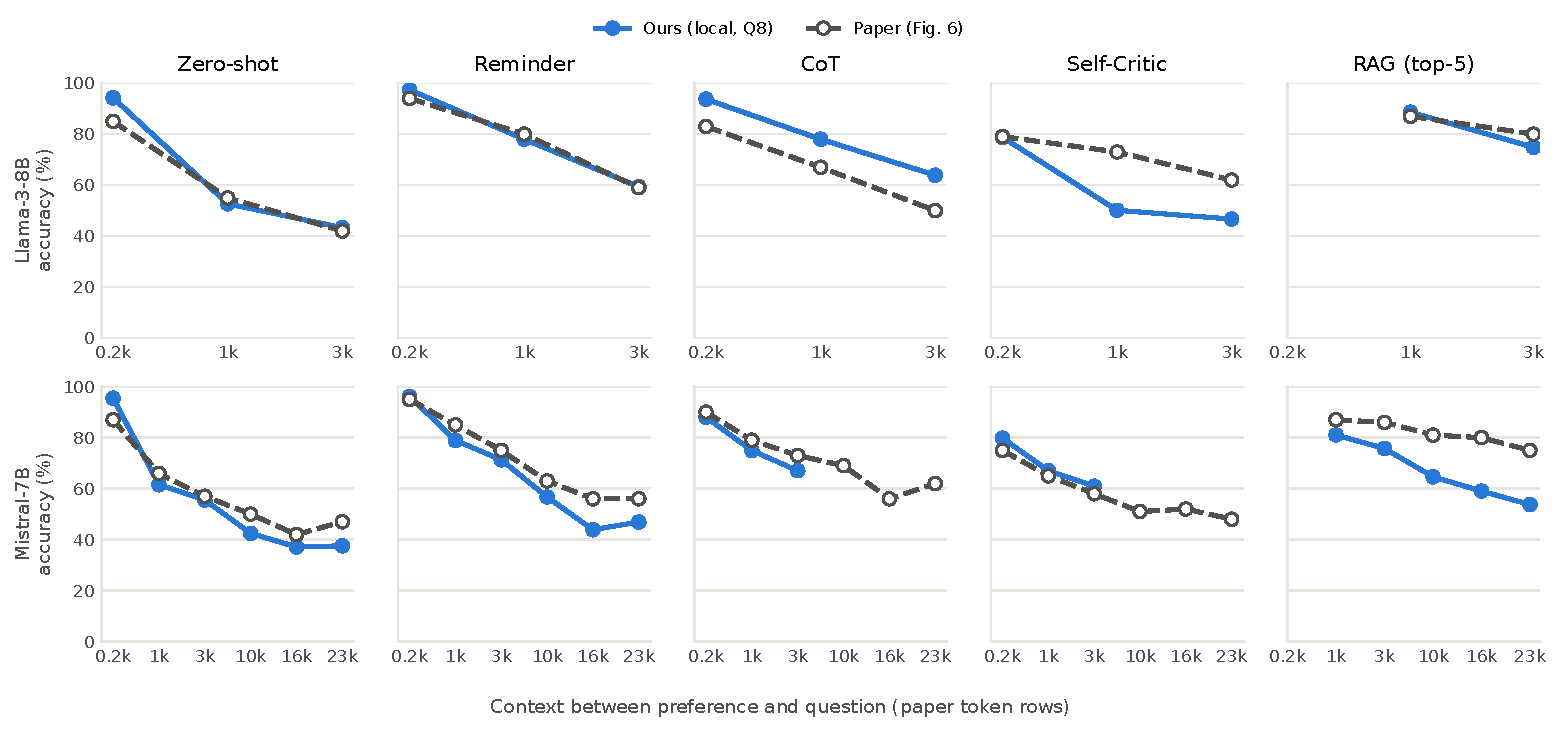
\includegraphics[width=0.83\linewidth]{fig_vs_paper.pdf}
\takeaway{Excluding 0.2k: \nWithinFive/\nCompared{} cells within 5 points of the paper, \nWithinTen/\nCompared{} within 10 (median gap \medianAbsDelta). Qualitative trends reproduce.}
\end{frame}

%-------------------------------------------------------------------------------
\begin{frame}{Where we differ, and why}
\begin{itemize}
  \item \textbf{Zero-shot, Reminder}: close up to 3k; 8--9 points \emph{higher} at 0.2k (easy setting)
  \item \textbf{CoT}: Llama +11 to +14, Mistral $-2$ to $-6$ $\rightarrow$ differences in model serving, not a pipeline bias
  \item \textbf{Self-Critic}: Mistral within 2--5 points; Llama $-15$ to $-23$ at 1k / 3k
    \begin{itemize}
      \item caused by the original Llama template: \llamaSCemptyOneK\% empty revisions at 1k
      \item excluding them: 78.8 / 67.1 / 47.8 (paper 79 / 73 / 62)
    \end{itemize}
  \item \textbf{RAG}: Llama matches; Mistral falls further below the paper as context grows ($-6$ $\rightarrow$ $-21$)
    \begin{itemize}
      \item plausible cause: 8-bit KV cache at long context (not yet verified)
    \end{itemize}
\end{itemize}
\end{frame}

%-------------------------------------------------------------------------------
\begin{frame}{Long context: Mistral-7B up to 23k tokens}
\begin{columns}[c]
\begin{column}{0.58\textwidth}
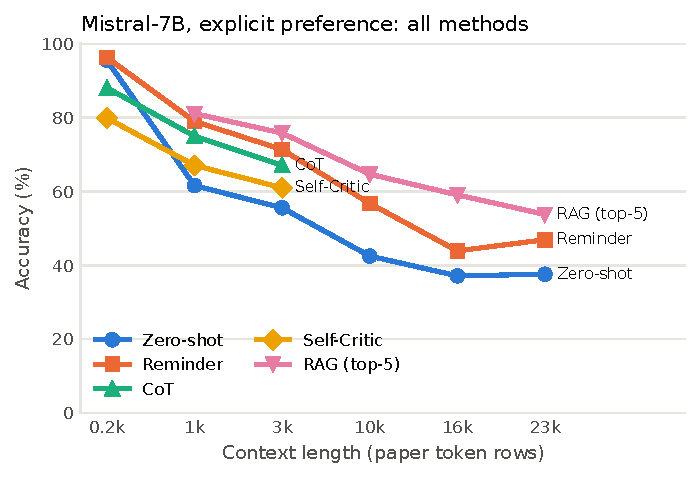
\includegraphics[width=\linewidth]{fig_mistral_long.pdf}
\end{column}
\begin{column}{0.42\textwidth}
\begin{itemize}
  \item Steep drop from 0.2k to 10k, then flat
  \item Reminder $>$ Zero-shot at every length
  \item RAG best throughout (53.7\% vs.\ 37.6\% at 23k)
  \item \textbf{Lesson}: a 3-topic pilot gave $\approx$23\% (chance level). Those topics were the hardest; all 20 topics are needed
\end{itemize}
\end{column}
\end{columns}
\end{frame}

%-------------------------------------------------------------------------------
\begin{frame}{Implicit (choice-based) preferences: new classification baselines}
\begin{columns}[c]
\begin{column}{0.6\textwidth}
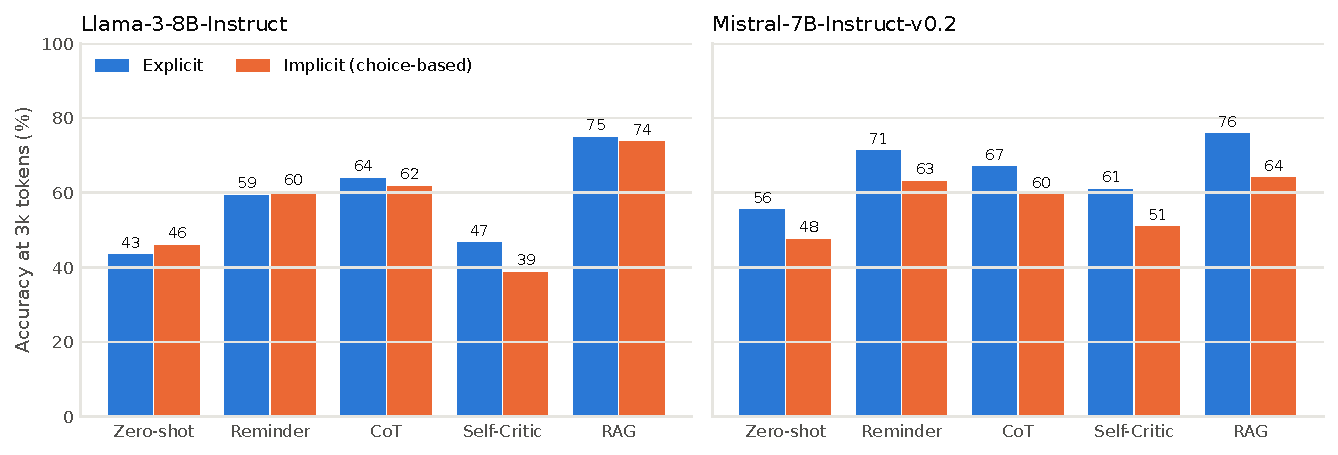
\includegraphics[width=\linewidth]{fig_explicit_vs_implicit.pdf}
\end{column}
\begin{column}{0.4\textwidth}
\begin{itemize}
  \item The paper reports implicit forms only for the generation task, so these are our own baselines
  \item Mistral: 7--15 points harder everywhere
  \item Llama: harder mainly at 0.2k; at 3k within 3 points for most methods
  \item These are the reference numbers for Phase 3
\end{itemize}
\end{column}
\end{columns}
\end{frame}

%-------------------------------------------------------------------------------
\begin{frame}{Finding 1: self-critique overturns correct answers}
\centering
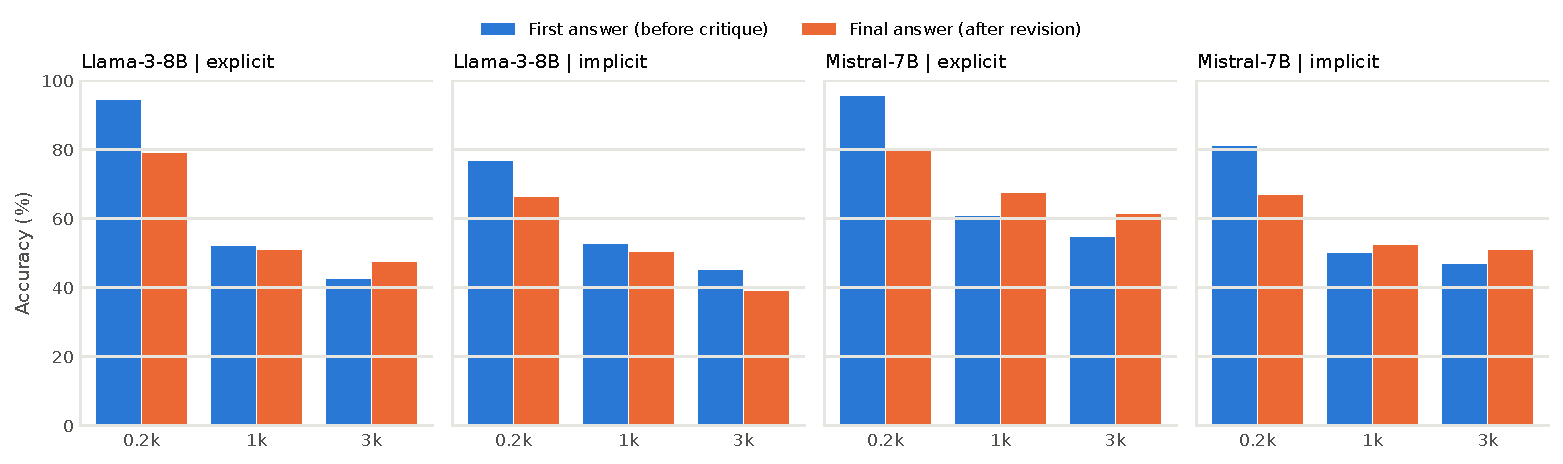
\includegraphics[width=0.9\linewidth]{fig_selfcritic.pdf}
\begin{itemize}
  \item At 0.2k: Llama \llamaSCrtwZero{} right$\rightarrow$wrong vs.\ \llamaSCwtrZero{} wrong$\rightarrow$right; Mistral \mistralSCrtwZero{} vs.\ \mistralSCwtrZero
  \item At longer contexts the net effect ranges from $-6$ to $+7$ points; this matches the paper's observation for classification
\end{itemize}
\end{frame}

%-------------------------------------------------------------------------------
\begin{frame}{Finding 2: at long context the model falls back on answer position}
\centering
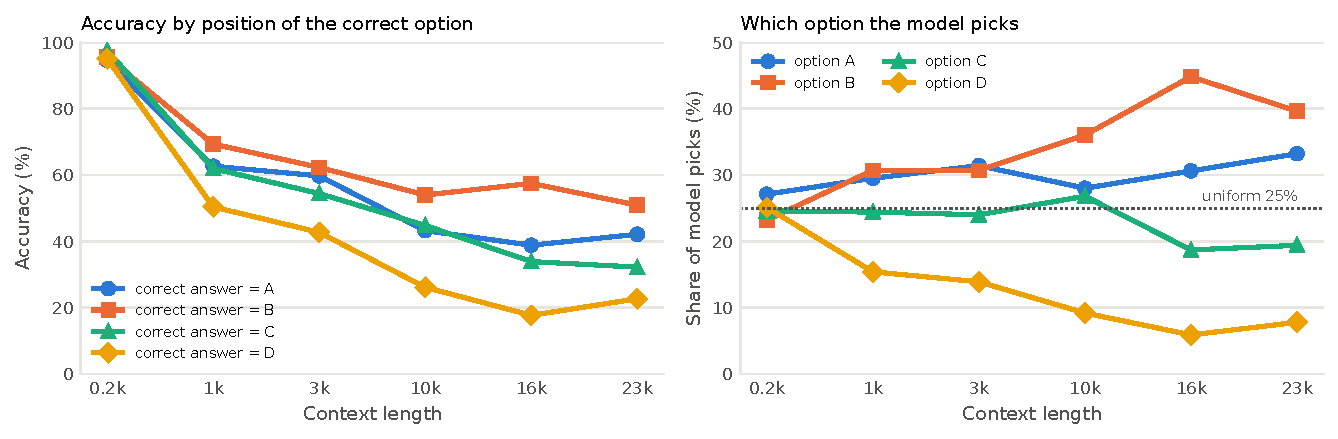
\includegraphics[width=0.82\linewidth]{fig_position_bias.pdf}
\begin{itemize}
  \item Accuracy when the correct answer is A vs.\ D: \posAccAthree\% vs.\ \posAccDthree\% at 3k; \posAccAlong\% vs.\ \posAccDlong\% at 23k
  \item The model favours B and avoids D (picked only \posPickDlong\% of the time at 23k). Once the preference is lost, a position prior remains
\end{itemize}
\end{frame}

%-------------------------------------------------------------------------------
\begin{frame}{Finding 3: retrieved context triggers refusals; topics differ widely}
\begin{columns}[c]
\begin{column}{0.48\textwidth}
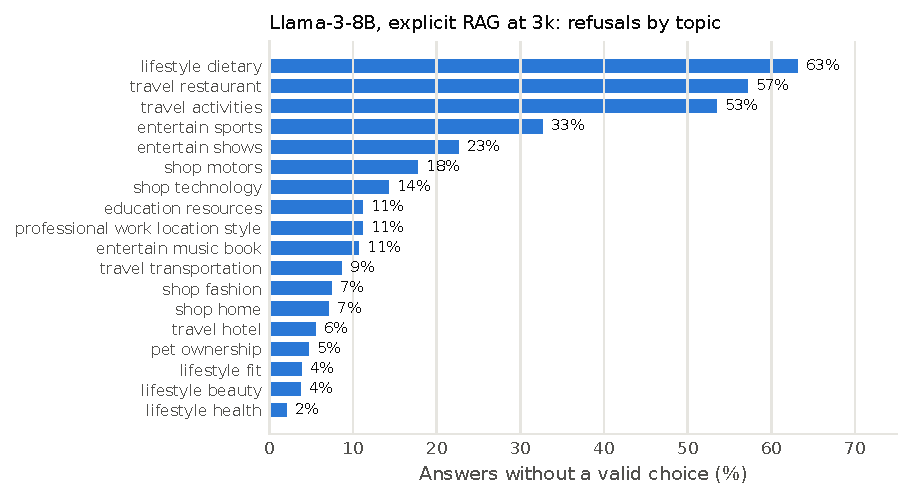
\includegraphics[width=\linewidth]{fig_rag_refusals.pdf}
{\footnotesize Llama RAG at 3k: \llamaRagRefusalAll\% answers without a choice, mostly refusals (\emph{``I cannot recommend\dots''}); Mistral 0.6\%}
\end{column}
\begin{column}{0.5\textwidth}
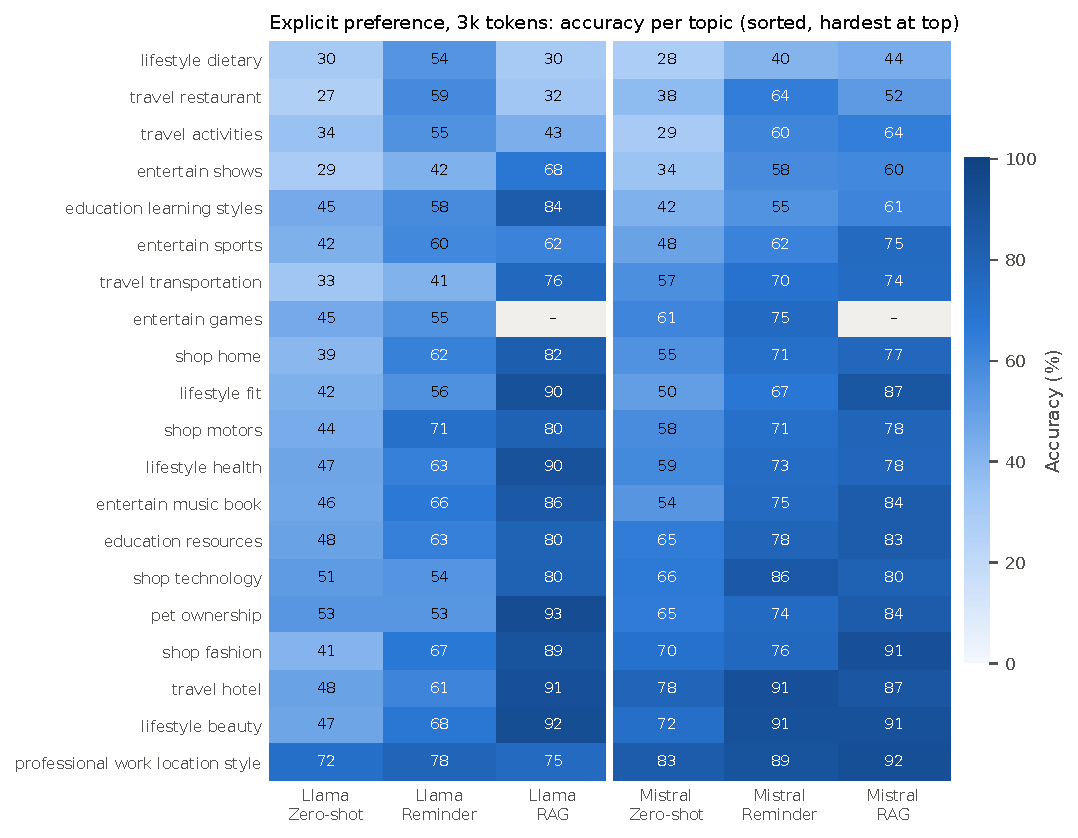
\includegraphics[width=\linewidth,height=0.76\textheight,keepaspectratio]{fig_topic_heatmap.pdf}
\end{column}
\end{columns}
\end{frame}

%-------------------------------------------------------------------------------
\begin{frame}{Deviations and threats to validity}
\begin{itemize}
  \item 8-bit weights on llama.cpp (vs.\ full precision on Bedrock); Mistral also uses an 8-bit KV cache
  \item Two prompt normalisations (start token, trailing whitespace); all prompt text is unchanged
  \item Per-question option shuffle (paired across methods, resumable)
  \item RAG coverage limited by data defects (19 topics explicit; 973/1000 implicit)
  \item One deterministic run per cell; binomial standard error $\le$ 1.6 points per cell
  \item Classification task only; the generation task needs an LLM judge
\end{itemize}
\vspace{6pt}
\centering\scriptsize
\begin{tabular}{lrrr}
\toprule
Runs & Questions & GPU hours & s / question \\
\midrule
Llama explicit (Tiers A+B) & 13,751 & 9.0 & 2.3 \\
Llama implicit-choice & 13,901 & 7.6 & 2.0 \\
Mistral explicit, short (Tiers A+B) & 13,853 & 8.6 & 2.2 \\
Mistral explicit, long (10k--23k) & 8,847 & 36.3 & 14.8 \\
Mistral implicit-choice & 13,931 & 9.8 & 2.5 \\
Smoke tests / checks & 195 & 0.1 & 2.7 \\
\midrule
Total & 64,478 & 71.4 & 4.0 \\
\bottomrule
\end{tabular}

\end{frame}

%-------------------------------------------------------------------------------
\begin{frame}{Feasibility and next steps}
\begin{columns}[T]
\begin{column}{0.5\textwidth}
\textbf{Phase 2: classifier}
\begin{itemize}
  \item Positives: explicit preference sentences and preference-revealing implicit turns
  \item Negatives: LMSYS turns and other dialogue turns
  \item \textbf{Topic-level split} to avoid leakage into Phase 3
  \item DistilBERT / ModernBERT / MiniLM; P/R per form, latency
\end{itemize}
\end{column}
\begin{column}{0.5\textwidth}
\textbf{Phase 3: full pipeline}
\begin{itemize}
  \item Classifier $\rightarrow$ memory, plus bge / e5 retrieval
  \item Same runner, prompts and settings guard as the baselines
  \item Targets: the 0.2k$\rightarrow$3k drop, the position-prior collapse, RAG refusals
\end{itemize}
\textbf{Scope changes}
\begin{itemize}
  \item Long regime via Mistral; Mixtral dropped (hardware)
  \item Generation task / proprietary model on a small subset, depending on API budget
\end{itemize}
\end{column}
\end{columns}
\end{frame}

%-------------------------------------------------------------------------------
\begin{frame}{Summary}
\begin{itemize}
  \item PrefEval's classification benchmark now runs \textbf{fully locally} with the original prompts, and is resumable and logged
  \item \nQuestions{} questions: 2 paper models $\times$ 5 methods $\times$ 2 preference forms $\times$ up to 6 context lengths
  \item The paper's findings reproduce; most numbers are within a few points, and the larger gaps have identified or plausible causes
  \item Found and fixed 3 prompt-formatting issues and 2 defects in the released data
  \item New observations (self-critique overturning answers, position-prior collapse, RAG refusals) give concrete targets for the classifier + memory pipeline
\end{itemize}
\vspace{10pt}
\centering\Large\textcolor{accent}{Thank you. Questions?}
\end{frame}

\end{document}
